

\begin{frame}{NUMA-aware MPI Model}
  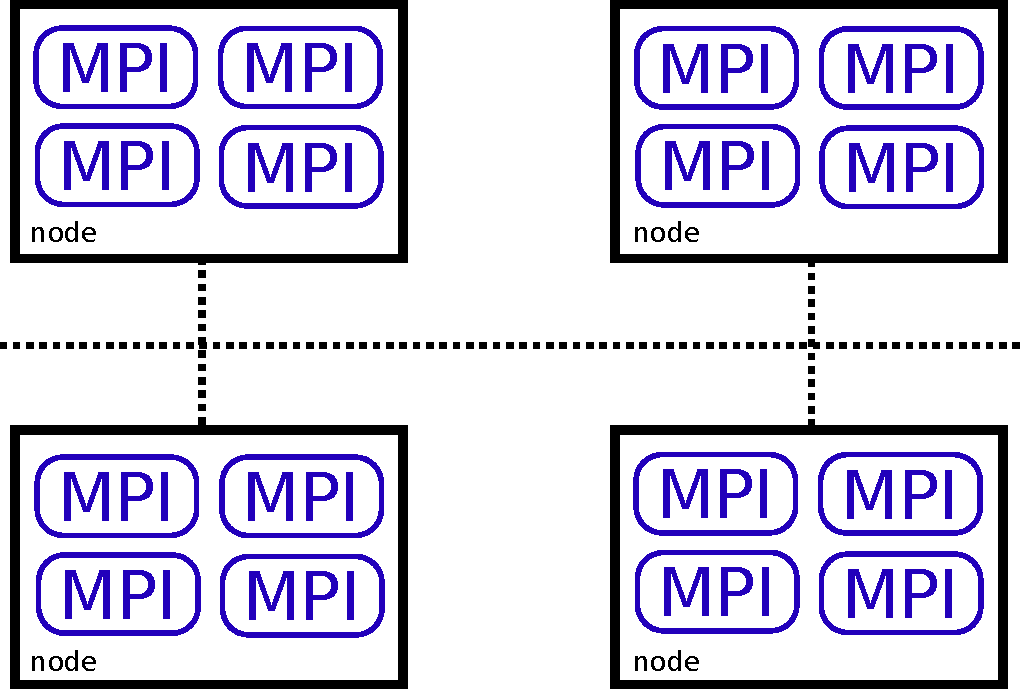
\includegraphics[width=1.0\textwidth]{figures/numa-mpi}
\end{frame}


%%%%%%%%%%%%%%%%%%%%%%%%%%%%%%%


%% Memory bandwidth vs. Parallelism

\begin{frame}[fragile]{Memory Bandwidth vs. Parallelism}
 \begin{center}
  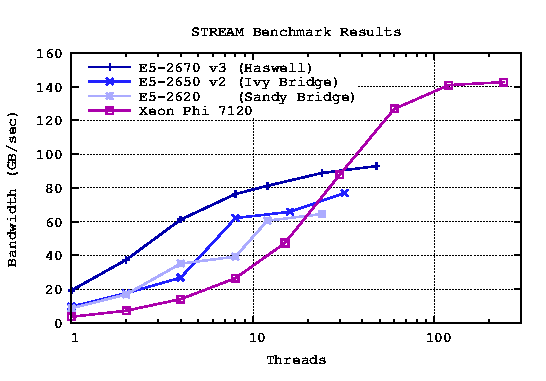
\includegraphics[width=0.95\textwidth]{figures/stream}
 \end{center}
 {\scriptsize https://www.karlrupp.net/2015/02/stream-benchmark-results-on-intel-xeon-and-xeon-phi/ }
\end{frame}



%%%%%%%%%%%%%%%%%%%%%%%%%%%%%%%


\begin{frame}[fragile]{Threads and Library Interfaces}

 \begin{block}{Attempt 1}
  \begin{itemize}
   \item Library spawns threads
  \end{itemize}
 \end{block}

   \begin{lstlisting}
  void library_func(double *x, int N) {
    #pragma omp parallel for
    for (int i=0; i<N; ++i) x[i] = something_complicated();
  }
  \end{lstlisting}

  \begin{block}{Problems}
   \begin{itemize}
    \item Call from multi-threaded environment?
   \begin{lstlisting}
  void user_func(double **y, int N) {
    #pragma omp parallel for
    for (int j=0; j<M; ++j) library_func(y[j], N);
  }
  \end{lstlisting}
    \item Incompatible OpenMP runtimes (e.g. GCC vs. ICC)
   \end{itemize}
 \end{block}

\end{frame}

\begin{frame}[fragile]{Threads and Library Interfaces}

 \begin{block}{Attempt 2}
  \begin{itemize}
   \item Use pthreads/TBB/etc. instead of OpenMP to spawn threads
   \item Fixes incompatible OpenMP implementations (probably)
  \end{itemize}
 \end{block}

  %\pause
  \begin{block}{Problems}
   \begin{itemize}
    \item Still a problem with multi-threaded user environments
   \begin{lstlisting}
  void user_func(double **y, int N) {
    #pragma omp parallel for
    for (int j=0; j<M; ++j) library_func(y[j], N);
  }
   \end{lstlisting}
  \end{itemize}
 \end{block}

\end{frame}


\begin{frame}[fragile]{Threads and Library Interfaces}

 \begin{block}{Attempt 3}
  \begin{itemize}
   \item Hand back thread management to user
  \end{itemize}
 \end{block}

  \begin{lstlisting}
  void library_func(ThreadInfo ti, double *x, int N) {
    int start = compute_start_index(ti, N);
    int stop  = compute_stop_index(ti, N);
    for (int i=start; i<stop; ++i)
      x[i] = something_complicated();
  }
  \end{lstlisting}

  %\pause
  \begin{block}{Implications}
   \begin{itemize}
    \item Users can use their favorite threading model
    \item API requires one extra parameter
    \item Extra boilerplate code required in user code
  \end{itemize}
 \end{block}

\end{frame}


\begin{frame}[fragile]{Threads and Library Interfaces}

 \begin{block}{Reflection}
  \begin{itemize}
   \item Extra thread communication parameter
    \begin{lstlisting}
void library_func(ThreadInfo ti, double *x, int N) {...}
    \end{lstlisting}
    %\pause
   \item Rename thread management parameter
    \begin{lstlisting}
void library_func(Thread_Comm c, double *x, int N) {...}
    \end{lstlisting}
    %\pause
   \item Compare:
    \begin{lstlisting}
void library_func(MPI_Comm comm, double *x, int N) {...}
    \end{lstlisting}
  \end{itemize}
 \end{block}

 %\pause
  \begin{block}{Conclusion}
   \begin{itemize}
    \item Prefer flat MPI over MPI+OpenMP for a composable software stack
    \item MPI automatically brings better data locality
  \end{itemize}
 \end{block}

\end{frame}
